\chapterimage{./Images/head2.jpg} % Chapter heading image
\chapter{Diodes - Chapter 4 of the Textbook}


\begin{definition}
    [Diode]
    \begin{itemize}
        \item Two-terminal device
        \item Allows current to flow in one direction only
        \item Non-linear device
    \end{itemize}
    % tikz code for diode with positive and negative terminals
    \begin{figure}[H]
        \centering
        \begin{circuitikz}
            \draw (0,0) to[diode] (2,0)
            (0,0) node[anchor=east] {Anode +}
            (2,0) node[anchor=west] {- Cathode};
        \end{circuitikz}
        \caption{Diode}
    \end{figure}
    % Cathode V-I characteristics
    \begin{figure}[H]
        \centering
        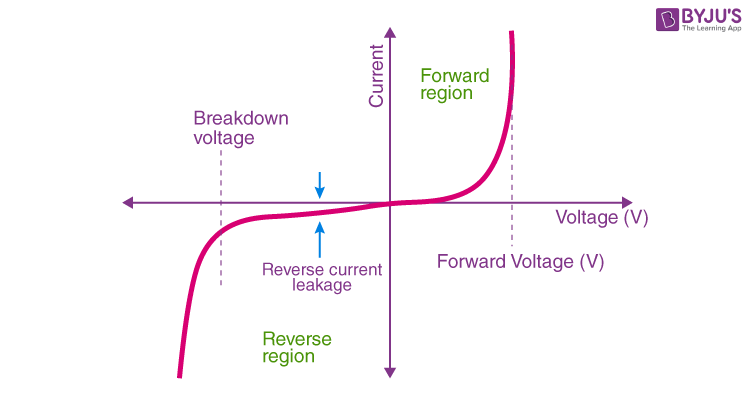
\includegraphics[scale=0.5]{./LECTURE_1/vi_diode.png}
        \caption{True Diode V-I Characteristics}
    \end{figure}
\end{definition}

\subsection*{Models of Voltage-Current Characteristics in Diodes}
\begin{definition}
    [Ideal Diode Model]
    \begin{itemize}
        \item Ideal diode has zero resistance and infinite current when forward biased (positive voltage)
        \item Ideal diode has infinite resistance and zero current when reverse biased (negative voltage)
        \item We assume we don't get to the breakdown voltage
    \end{itemize}
    % tikz code for ideal diode V-I characteristics
    \begin{figure}[H]
        \centering
        \begin{tikzpicture}
            \begin{axis}[
                    axis lines = left,
                    xlabel = $V$,
                    ylabel = $I$,
                    xmin = -1,
                    xmax = 1,
                    ymin = -1,
                    ymax = 1,
                ]
                %Below the red parabola is defined
                \addplot [
                    domain=-1:1,
                    samples=100,
                    color=red,
                ]
                {x < 0 ? 0 : 10};
            \end{axis}
        \end{tikzpicture}
        \caption{Ideal Diode V-I Characteristics}
    \end{figure}

\end{definition}

\begin{corollary}
    [Analysis Using Ideal Diode Model]
    \begin{itemize}
        \item If the diode is forward biased, replace the diode with a short circuit
        \item If the diode is reverse biased, replace the diode with an open circuit
    \end{itemize}
    % circuit diagram with ideal diode
    \begin{figure}[H]
        \centering
        \begin{minipage}{0.3\textwidth}
            \centering
            \begin{circuitikz}[scale=0.8]
                \draw
                (0,0) to[battery1, l=$V$] (0,4)
                (0,4) to[diode, l=$D$] (4,4)
                (4,4) to[R, l=$R$] (4,0)
                (4,0) -- (0,0);
            \end{circuitikz}
            \caption{Ideal Diode}
        \end{minipage}
        \hfill
        \begin{minipage}{0.3\textwidth}
            \centering
            \begin{circuitikz}[scale=0.8]
                \draw
                (0,0) to[battery1, l=$V$] (0,4)
                (0,4) to[short, -o] (1,4)
                (4,4) to[short, -o] (3,4)
                (4,4) to[R, l=$R$] (4,0)
                (4,0) -- (0,0);
            \end{circuitikz}
            \caption{Forward Biased Diode}
        \end{minipage}
        \hfill
        \begin{minipage}{0.3\textwidth}
            \centering
            \begin{circuitikz}[scale=0.8]
                \draw
                (0,0) to[battery1, l=$V$] (0,4)
                (0,4) -- (4,4)
                (4,4) to[R, l=$R$] (4,0)
                (4,0) -- (0,0);
            \end{circuitikz}
            \caption{Reverse Biased Diode}
        \end{minipage}
    \end{figure}
\end{corollary}


\begin{definition}
    [Piecewise Linear Model]
    \begin{itemize}
        \item Diode has a forward voltage drop $V_f$ and a reverse saturation current $I_s$
        \item $V_f$ is the voltage at which the diode starts conducting
        \item $I_s$ is the current when the diode is reverse biased
    \end{itemize}
    % tikz code for piecewise linear diode V-I characteristics
    \begin{figure}[H]
        \centering
        \begin{tikzpicture}
            \begin{axis}[
                    axis lines = left,
                    xlabel = $V$,
                    ylabel = $I$,
                    xmin = -1,
                    xmax = 1,
                    ymin = -1,
                    ymax = 1,
                ]
                %Below the red parabola is defined
                \addplot [
                    domain=-1:1,
                    samples=100,
                    color=red,
                ]
                {x < 0 ? 0 : x};
            \end{axis}
            \draw[dotted] (3.5,0) -- (3.5,2.8) node[right] {$V_f$};
        \end{tikzpicture}
        \caption{Piecewise Linear Diode V-I Characteristics}
    \end{figure}

\end{definition}